\documentclass{article}
\usepackage{graphicx}	% for including graphics files
\usepackage{ifpdf}	% use same .tex file for both latex & pdflatex
\usepackage{amsmath}
\usepackage{subcaption}	% allow multiple images
%\usepackage[export]{adjustbox}  allows left, right, inner image positioning

\ifpdf
  \usepackage[colorlinks,linkcolor=blue,urlcolor=blue,citecolor=blue,plainpages=false,pdfpagelabels,breaklinks]{hyperref}
\else
  \usepackage[colorlinks,linkcolor=blue,urlcolor=blue,citecolor=blue,plainpages=false,pdfpagelabels,linktocpage]{hyperref}
\fi

\title{my title}
\date{2018-02-14}
\author{Gao Zhiyuan}

% preamable is the area before document

\begin{document}
  \pagenumbering{gobble}	% no page number
  \maketitle
%  \newpage
  \pagenumbering{arabic}	% count page from here, roman-roman numbers

  \section{title of Section}
  Hello World!
  \subsection{subsection}
  a subsection
  \subsubsection{subsubsection}
  a subsubsection 
  \paragraph{paragraph}
  this is a paragraph
  \subparagraph{subparagraph}
  this is a subparagraph

  \section{Another section}

  \begin{equation}
	  f(x) = x^2
  \end{equation}

\begin{equation*}	% remove auxiliary calculation
	  f(x) = x^2
  \end{equation*}

  \section{inline math}

  formula: $f(x) = x^2$

  \begin{align*}
	  1 + 2 &= 3 \\ 
	  1 &= 3 - 2
  \end{align*}


  align environment will align the equations at the ampersand 



  single formulas must be seperated with two backslashes
%  \\ linebreak

%  asterisk * indicates that I don't want the equations to be numbered


 \begin{align*}
	     f(x) &= x^2\\
	     g(x) &= \frac{1}{\sqrt{x}}\\
	     F(x) &= \int^a_b \frac{1}{3}x^3
 \end{align*}


 Matrices only work within math dollar signs $
 	\begin{matrix}
		 1 & 0\\
		 1 & 1
	 \end{matrix}
 $

 $
 [
	 \begin{matrix}
		 1 & 0\\
		 0 & 1
	 \end{matrix}
 ]
 $

$\left( \frac{1}{\sqrt{x}} \right)$

$\lambda$


\section{pictures}


\begin{figure}[h!]
	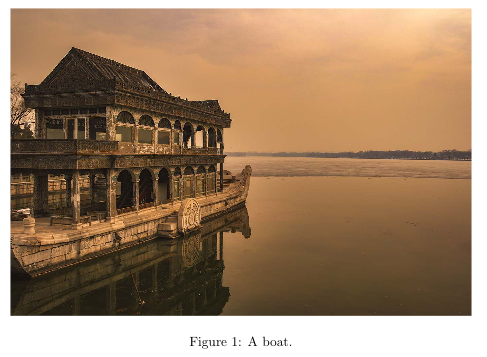
\includegraphics[width=\linewidth]{boat.jpg}
	% \linewidth: picture will be scaled to fit width of the document
	% width=0.5\textwidth could be a choice
	\caption{A boat.}
	\label{fig:boat1}
\end{figure}

Figure \ref{fig:boat1} shows a boat.

% \begin{figure}[h!]
	% h(here)
	% t(top)
	% b(bottom)
	% p(page)
	% !(override) - force the specified location
% \end{figure}

\begin{figure}[h!]
  \centering
  \begin{subfigure}[b]{0.4\linewidth}
  
\includegraphics[width=\linewidth]{coffee.jpg}
  \caption{Coffee.}
  \end{subfigure}
  \begin{subfigure}[b]{0.4\linewidth}
  
\includegraphics[width=\linewidth]{coffee.jpg}
  \caption{More coffee.}
  \end{subfigure}
  \caption{The same cup of coffee. Two times.}
  \label{fig:coffee}
\end{figure}

\newpage
\tableofcontents
\section{section}
Dummy text
\subsection{subsection}
Dummy text


\end{document}


